The suggested framework has a total of 8 phases in the classification pipeline which is mentioned in the image presented in table 1.0. The experiments were performed in three scenarios that included pre-training the transfer-learning models on the imageNet, hisbrek dataset and with the random weight initialization in order to evaluate the performance
of each of the models with both partial and complete fine-tuning applied to the target models.

\section{Image Segmention and Preprocessing}
The first phase, targets to obtain the segmented regions of interests from the target source image. 
In order to perform the image segmentation of the source images of 
histopathological images, the pre-processing procedure was performed which involves 
the following sub-procedures which includes color channel separation and 
image normalization and explained in the detailed manner.
\pagebreak
\subsection{Color Channel Seperation}
\begin{figure}[!htp]
    \centering
    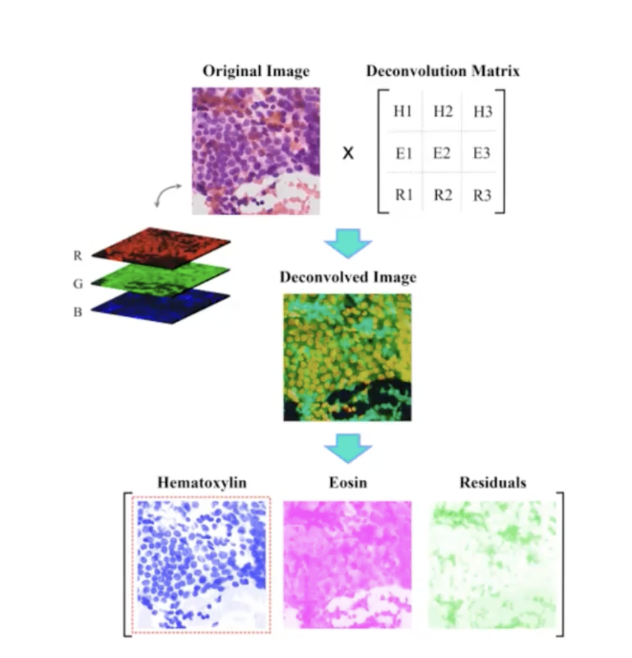
\includegraphics[scale=0.75]{assets/pre-processing.png}
    \caption{Image Credits: MSC Thesis Examination (Presentation) - Mohammad Amin Shamshiri}
\end{figure}
Color channel separation as shown in the figure[1.2] which aims at decomposing three color channels of the nucleus rather than the other components which are present within the image. In order to perform the color channel separation task, 
the deconvolutional matrix was applied to extract the feature maps of three distinct kinds that involve hematoxylin, Eosin and residuals. Upon investigation, the hematoxylin feature maps were most prominent and were used for the further normalization and segmentation. 


\subsection{Image normalization}
The normalization of the images are performed in order to ensure that the images are easier to process and each pixel in the image is normalized to range within 0 and 1 pixel values rather than 0 and 255, which is easier to train on the convolutional neural networks \citep{rashid_2019}.  

\subsection{Problems with using the UNET segmentation }
In the early phase of the experiments, the semantic segmentation was performed on the hematoxlyin images with an objective of grouping the each pixel in the images into the group of nuclei-interior, nuclei-edge or the background using the famous U-Net model, which requires the manual segmentation of the images and that is very time consuming process.
The subset of the original dataset was used to evaluate the performance of the segmented images upon splitting the dataset into the training and validation datasets respectively. 
However, the quantitative analysis of the U-Net segmentation was not possible and can only be evaluated on the visual basis. 
Therefore as for further investigation the intensity thresholding technique has been opted to deal with such problems and provide a reliable mechanism for image segmentation. 